\documentclass[a4paper,12pt]{report}
\usepackage[cm-default]{fontspec}

%Требуется для русского языка
\usepackage[russian]{babel}

%Отступы в документе
\usepackage[top=20mm, bottom=20mm, left=25mm, right=15mm]{geometry}
 
%\usepackage{xunicode, xltxtra}

%Требуется для некоторых символов и ссылок на выражения \eqref
\usepackage{amsmath}

%Требуется для гиперссылок по документу 
\usepackage{hyperref}

%Требуется для обозначений модуля, округления вверх и вниз
\usepackage{mathtools}

%Требуется для флага [H] для фиксации позиции графика в документе
\usepackage{float}

%Требуется для импорта изображений
\usepackage{graphicx}

%Построение графиков
\usepackage{pgfplots}
\pgfplotsset{compat=1.9}

%Разметка алгоритмов
\usepackage[ruled, vlined]{algorithm2e}

%Для римских цифр в enumerate
\usepackage{enumitem}

%Собственные функции (с использованием mathtools) для заключения в модуль или округления
\DeclarePairedDelimiter\ceil{\lceil}{\rceil}
\DeclarePairedDelimiter\floor{\lfloor}{\rfloor}
\DeclarePairedDelimiter\abs{\lvert}{\rvert}%

%Установка шрифта
\setmainfont{Times New Roman} 

%Цвета в титульном листе
\usepackage{multicol}
\usepackage{color}

\definecolor{darkgreen}{rgb}{0, 0.5, 0}
\definecolor{graylight}{rgb}{0.6, 0.6, 0.6}

\begin{document}

\thispagestyle{empty}

\begin{center}

\sc
ФЕДЕРАЛЬНОЕ  ГОСУДАРСТВЕННОЕ АВТОНОМНОЕ
ОБРАЗОВАТЕЛЬНОЕ УЧРЕЖДЕНИЕ ВЫСШЕГО ОБРАЗОВАНИЯ
«НАЦИОНАЛЬНЫЙ ИССЛЕДОВАТЕЛЬСКИЙ УНИВЕРСИТЕТ
«ВЫСШАЯ ШКОЛА ЭКОНОМИКИ»
\end{center}

\begin{center}
\bf Московский институт электроники и математики им.~А.Н.~Тихонова
\end{center}

\vspace{1cm}

\begin{center}
Дородный Дмитрий Алексеевич
\end{center}

\vspace{1cm}

\begin{center}
\bf Перевод статьти Роберта Сильвермана  "Мультиполиномиальное квадратичное решето"
\end{center}

\vspace{10mm}

\begin{center}
Курсовая работа \par
по специальности 10.05.01 «Компьютерная безопасность» \par
студента образовательной программы специалитета
\end{center}

\vfill

\begin{multicols}{2}
\begin{flushleft}
~Студент\par\:\par
\begin{tabular}{c}
\underline{\hspace{8em}} \vspace{-2mm}\\
{\tiny {\color{graylight}подпись}}
\end{tabular}
\begin{tabular}{c}
\underline{\hspace{2em}Дородный Д.А.\hspace{1em}}\\
{\tiny{\color{graylight} ФИО}}
\end{tabular}
\end{flushleft}

\begin{flushright}
Преподаватель

доцент
\end{flushright}

\begin{tabular}{c}
\underline{\hspace{8em}} \vspace{-1mm}\\
{\tiny {\color{graylight}подпись}}
\end{tabular}
\begin{tabular}{c}
\underline{\hspace{2em}Нестеренко А.Ю.\hspace{1em}} \vspace{-1mm}\\
{\tiny{\color{graylight} ФИО}}
\end{tabular}
\end{multicols}

\vfill
\begin{center}Москва, 2021 г.\end{center}

\newpage

\tableofcontents


\begin{abstract}

Обсуждается модификация Петером Монтгомери алгоритма факторизации больших целых чисел с использованием квадратичного решета, а также ее реализации. Использование модификации позволяет факторизацию с на порядок меньшим количеством просеивания, чем в базовом алгоритме. Она позволяет факторизовать числа в диапазоне 60 десятичных знаков за день, используя большой миникомпьютер. Алгоритм обладает свойствами, которые делают его хорошо адаптируемым к распараллеливанию.
\end{abstract}


\section{Введение}
Базовый алгоритм квадратичного решета имеет корни, которые отсылают к М. Краичику, однако явно заявил и проанализировал алгоритм С. Померанц. Было всего две реализации данного алгоритма, первая Дж. Гервером в Рутгерсе, а вторая Дж. Дэвисом и Д. Холдриджем в Национальных Лабораториях Сандия. Последние использовали компьютер Cray-1 чтобы факторизовать числа в диапазоне 60-70 десятичных знаков из ''Проекта Каннингхема''. Они также использовали Cray XMP чтобы разложить на множители тогда еще ''разыскиваемое'' число $(10^{71} -1)/9$ за 9 с половиной часов. И тогда как некоторые аргументы по теме были уже освещены Померанцем \cite{pomer}, мы представляем нашу статью как более ориентированную в сторону реализации алгоритма. Базовый алгоритм строится на составлении решения к следующему уравнению, где $N$ - число, которое требуется факторизовать.

\begin{equation}\label{eq:1}
A^2 \equiv B^2 \mod N
\end{equation}

Если $A \not\equiv B \mod N$ и $A \not\equiv -B \mod N$, тогда $(A + B), N$ и $(A - B, N)$ - делители $N$.

Эта версия квадратичного решета генерирует набор квадратичных вычетов $N$, используя следующий многочлен:

\begin{equation}\label{eq:2}
Q(x) = (x + [\sqrt{N}])^2 - N \equiv H^2 \mod N.
\end{equation}

Сразу становится очевидно, что если простое число $p | Q(x)$, тогда $p | Q(x + kp)$ для всех $k \in $. Таким образом, значения многочлена можно профакторизовать с помощью решета, когда мы решаем $Q(x) \equiv 0 \mod p$. Это выражение может быть решено любым из числа доступных алгоритмов \cite[стр 437]{knuth}. Потенциальные делители $p$ из $Q(x)$ в точности те простые чсла, символ Лежандра которых $(N/p) = 1$ и элемент $-1$ нужен, чтобы хранить знак. 
Теперь алгоритм продолжается следующим образом:

\begin{enumerate}[label=\roman*]
	\item Выбрать факторную базу $FB = {p_i | (N/p) = 1, p_i, prime, i = 1, \ldots, F}$ для какого-то подходящего значения $F$, и $p_0 = 1$ для знака.
	\item Решить квадратное уравнение $Q(x) \equiv 0 \mod p_i$ для всех $p_i \in FB$. Для каждого из $p_i$ будет найдено два корня: $r_1, r_2$.
	\item Инициализировать массив просеивания нулями на интервале $[-M, M]$ для какого-то подходящего $M$.
	\item Для всех $p_i \in FB$ прибавить значение $[log(p_i)]$ к ячейкам массива в индексах: $r_1, r_1 \pm p_i, r_1 \pm 2p_i, \ldots$ затем $r_2, r_2 \pm p_i, p_2 \pm 2p_i, \ldots$
	\item Значение $Q(x)$ будет примерно $M\sqrt{N}$ на $[-M, M]$, так что сравниваем каждую ячейку с  $[\log{N}/2 + \log{M}]$. Полностью факторизованные вычеты будут иметь их соответствтующее значение близким к этому. Для таких значений построим точную факторизацию перебором делителей. Факторизации находятся так редко, что временные затраты на эти переборы делителей незначительны. При подсчете не требуется проверять все простые числа в факторной базе. Если $x$ - ячейка в массиве просеивания, нужно только лишь вычислить $R \equiv x \mod p_i$. Только если $R$ равно одному из двух корней следует продолжить и выполнить многоточное деление:
\begin{equation}\label{eq:3}
Q(x) = \prod_{i = 0}^{F}p_i^{a_i}, p_i \in FB.
\end{equation}

Пусть $v_j$ - соответствующий вестор экспонент $[\alpha_{j1}, \alpha_{j2}, \alpha_{j3}, \ldots, \alpha_{jF}]$ с $H_{j}^2 = Q(x)$. 
	\item Насобирать $F+1$ факторизацию. Затем требуется найти набор вычетов, произведение которых является квадратом при помощи метода Гаусса над полем $GF(2)$ на матрице, полученной при приведении всех векторов $v_j$ по модулю 2. Это дает нам линейную зависимость по модулю 2 на степенях, и произведение векторов в этой зависимости дает квадрат. Затем, составление соотношения \eqref{eq:1} - тривиальная задача.

\end{enumerate}
Основная сложность этого подхода заключается в том, что необходимо насобирать количество вычетов, сопоставимое с количеством простых чисел в базе факторизации. Чтобы было возможно получить достаточно факторизаций, $M$ должно быть очень большое, и вычеты будут расти линейно пропорционально $M$. 

Обходной путь к этой проблеме был изначально предложен Петером Монтгомери. Просто использовать много многочленов, чтобы генерировать вычеты и просеивать каждый многочлен на намного меньшем интервале. Использование нескольких многочленов позволяет сохранить интервал просеивания довольно маленьким, что делает вычеты проще факторизуемыми. Мы применили этот подход и нашли его крайне эффективным. Он позволяет найти достаточно факторизованных остатков используя менее чем одну десятую чать от общей длины решета, используемого в версии с одним многочленом. Мы также показываем, что стоимость смены многочлена мала.

На самом деле, сандийская реализация была сделана в двух этапах. Их первая версия использовала один многочлен. Более поздняя версия использовала несколько многочленов, но в замаскированной а не в явной форме. Эта поздняя версия создавала неявные многочлены из подпоследовательностей основного решета, которое делилось на большое простое число $q$ вне факторной базы. Они назвали этот метода ''особые $q$''. Многочлены, предложенные Монтгомери в какой-то мере лучше, однако, потому что они производят вычеты, которые в среднем меньшие и более простые в реализации.

В секции 2 мы обсудим, как выбирать коэффициенты многочленов. Секция 3 покажет, как эффективно вычислять эти коэффициенты. В секции 4 обсудим базовые шаги алгоритма. Секция 5 расскажет о выборе различных входных параметров алгоритма. Секция 6 представит некоторые числовые результаты. В секции 7 поговорим о параллельной реализации и, наконец, в секции 8 сравним наш алгоритм с другими методами.

\section{Выбор коэффициентов}

Выберем $Q(x) = Ax^2 + Bx + C$. Для того, чтобы $Q(x)$ мог генерировать квадратичные вычеты, необходимо чтобы $B^2 - 4AC = N$. Так как последнее выражение сравнимо с 0 или 1 по модулю 4, это означает, что если $N \equiv 3 \mod 4$ необходимо сначала умножить $N$ на небольшую константу $k$, такую что $kN \equiv 1 \mod 4$. Вообще это хорошая практика, потому что обычно это позволяет построить факторную базу, в которой намного больше маленьких простых чисел. Мы позднее обсудим функцию, которая может быть использована для вычисления этого множителя $k$. Предложение Померанца \cite{pomer} позволяет ограничиться лишь следующим выражением: $kN \equiv 1 \mod 4$. Нужно всего лишь взять средний коэффициент $2B$ вместо $B$. Однако, мы еще не дошли до реализации этого предложения. Для нас будет преимуществом возможность сохранить отностильно малое значение $Q(x)$ в какой-то мере над [-M, M]. Есть несколько очевидных способов сделать это. Например,
\begin{subequations}
	\begin{align}
		&\text{Минимизируем} \sup |Q(x)| \text{на} [-M, M] \label{eq:4a} \\
		\text{или}\notag\\ 
		&\text{Минимизируем} \int_{-M}^{M} |Q(x)|dx  \label{eq:4b} \\
		\text{или}\notag\\ 
		&\text{Минимизируем} \int_{-M}^{M} {Q(x)}^2dx \label{eq:4c} \\
		\text{А также} \notag \\
		&B^2 - 4AC = kN \text{ и } A, B, C \in Z \label{eq:4d}
	\end{align}
	\label{eq:4all}
\end{subequations}

Легко заметить, что \eqref{eq:4a} и \eqref{eq:4b} практически эквивалентны. Длина основания параболы $2M$, и ее площадь будет прямо пропорциональна ее высоте. Уменьшая целочисленные ограничения и решая каждую из изложенных выше задач множителя Лагранжа, можно прийти к выводу, что все одни дают один и тот же результат. Точный ответ на \eqref{eq:4a}:

\begin{align}\label{eq:4}
&\mathrel{\phantom{=}}A = W_1\sqrt{kN}/M\notag\\
&\mathrel{\phantom{=}}B = 0\\
&\mathrel{\phantom{=}}C = W_2M\sqrt{kN}\notag
\end{align}

где

\begin{equation*}
W_1 = \sqrt{2}/2 \text{ и } W_2 = -1/2\sqrt{2}.
\end{equation*}

Единственное различие между результатами различными задачами минимизации это то, что константы $W_1, W_2$ слегка изменяются. $W_1$ изменяется в диапазоне от $.70$ до $.75$ и $W_2$  изменяется от $-.4$ до $-.3$ при $W_1W_2 = -\frac{1}{4}$.

Максимальное значение $Q(x)$ над $[-M, M]$ это $M\sqrt{kN}/2\sqrt{2}$, улучшение на порядок $\sqrt{8}$ относительно \eqref{eq:2} и ''особыми $q$'' многочленами в Сандии.

$B = 0$ непосредственно следует из соображений симметрии, но (4a) и (4c) дают похожие результаты для $A$ и $C$ потому что ограничение $B^2 - 4AC = kN$ сильно связывает форму $Q(x)$. Самый простой путь увидеть это - это осознать, что в корнях наклон графика будет $\pm \sqrt{kN}$. Нам бы очень хотелось сплющить параболу, но ограничение на дискриминант означает, что кривая должна иметь некоторую ''крутость''. Таким образом, мы не можем ничего поделать, кроме как двигать параболу вверх и вниз.

\section{Вычисление коэффициентов}

Простой метод для выбора $A, B$ и $C$ получается из метода для быстрого нахождения квадратных корней. Для удовлетворения (4d) необходимо чтобы

\begin{equation}\label{eq:6}
B^2 \equiv kN \mod 4A
\end{equation}

Пусть $A = D^2, (D/kN) = 1, D \equiv 3 \mod 4$ и $A \approx \sqrt{kN/2}/M$. Желательно, чтобы $D$ было простым, потому что если простое число из факторной базы делит $A$, то $Q(x) \equiv 0 \mod p$ имеет только один корень, и вероятность того, что $p | Q(x)$ на $[-M, M]$ падает с $2/p$ до $1/p$. Для практических целей достаточно, чтобы $D$ было только лишь возможно простым числом. Альтернативно, можно выбрать $D$ как произведение простых чисел не входящих в факторную базу, но его факторизация должна быть известна, чтобы можно было решить \eqref{eq:6}. Наша реализация принимает $D$ как возможно простое число. Чтобы найти коэффициенты, надо посчитать
\begin{subequations}
\begin{align}
	&\mathrel{\phantom{=}}h_0 \equiv {(kN)}^{(D-3)/4} \mod D, \label{eq:7a}\\
	&\mathrel{\phantom{=}}h_1 \equiv kNh_0 \equiv (kN)^{(D+1)/4} \mod D. \label{eq:7b}
\end{align}
\label{eq:7all}
\end{subequations}

тогда

\begin{equation}\label{eq:8}
h_1^2 \equiv kN(kN)^{(D-1)/2} \mod D \equiv kN \mod D, так как (D/kN) = 1
\end{equation}

Пусть

\begin{equation}\label{eq:9}
h_2 \equiv (2h_1)^{-1}[\frac{kN - h_1^2}{D}] \mod D
\end{equation}

Тогда имеем

\begin{equation}\label{eq:10}
B \equiv h_1 + h_2D \mod A
\end{equation}

и

\begin{equation}\label{eq:11}
B^2 \equiv h_1^2 + 2h_1h_2D + h_2^2D^2 \equiv kN \mod A
\end{equation}

Так как $B$ должно быть нечетным, если оно получилось четное - вычесть его из A.
Значение $(2h_1)^{-1} \mod D$ легко получается, так как $h_0 \equiv h_1^{-1} \mod D$ уже было посчитано. Также имеем 

\begin{equation}\label{eq:12}
C = [\frac{B^2 - kN}{4A}]
\end{equation}

Это не необходимо, на практике, действительно вычислять \eqref{eq:12}, так как значение $C$ на самом деле не требуется. Однако, вычисление можно провести для проверки других вычислений. Посчитаем и сохраним значение $1/2D \mod kN$ на потом. Это позволит нам быстро посчитать $Q(x)$ огда нам нужно найти факторизацию.
Как результат того, как мы выбирали $D$, мы также имеем
\begin{equation}\label{eq:13}
Q(x) \equiv H^2 \equiv (\frac{2Ax + B}{2D} \mod kN).
\end{equation}

Требуется некоторая осторожность: Если $x$ находится между действительными корнями $Q(x)$, тогда $Q(x)$ - отрицательное, и необходимо вычесть его значение из $kN$.

Стоимость нахождения коэффициентов по большей части зависит от нахождения возможно простого числа и проверки вычетом на $D$, подсчетом $h_1$ и $1/2h_1 \mod D$ и $1/2D \mod kN$.
Наконец, корни $Q(x) \mod p_i, p_i \in FB$ 

\begin{equation}\label{eq:14}
(-B \pm \sqrt{kN})(2A)^{-1} \mod p_i,
\end{equation}

так как $B^2 - 4AC$ инвариантно.

Большинство стоимости смены многочленов появляется в вычислении \eqref{eq:14}. Стоимость подсчета \eqref{eq:14} доминируется вычислением $1/2A \mod p_i$, что должно быть выполнено для всех простых чисел в базе факторизации. Даже с эффективным алгоритмом для выполнения этой операции, таким как расширенный алгоритм Эвклида, как правило приходится выполнять эти операции тысячи раз при смене многочленов. На SUN-3/75, для числа длиной 60 десятичных знаков и факторной базой из 3000 простых чисел, требуется $.9$ секунд чтобы посчитать все коэффициенты и $2.6$ секунд, чтобы посчитать все корни.

\section{Описание алгоритма}

Здесь мы показываем базовые шаги в алгоритме.
\begin{enumerate}[label=\roman*]
	\item  Выберем множитель $k$, такой что $kN \equiv 1 \mod 4$ и $kN$ богато на маленькие квадратичные вычеты. Мы предпочитаем $kN \equiv 1 \mod 8$, так как $2 \in FB$ только если это условие выполняется. \label{romi}
	\item Выберем размер факторной базы $F$, длину интервала просеивания $2M + 1$, и большую константу $T$. Предложения по поводу значений этих величин даны ниже. \label{romii}
	\item Посчитаем тестовое значение \label{romiii}
	\begin{equation*}
	[\log{\frac{M\sqrt{kN/2}}{p_{max}^T}}]
	\end{equation*}
Где $p_{max}$ - это наибольшее простое число из базы факторизации. Если $T \leq 2$, то когда бы значение в ячейке массива просеивания ни превосходило это тестовое значение, это будет означать, что значение соответствующего $Q(x)$ будет полностью факторизуемым. Если $T > 2$, тогда $Q(x)$ может не раскладываться полностью. Однако, эти частичные факторизации могут также быть полезными, как мы увидим далее.
	\item Посчитать факторную базу $FB$ и $\sqrt{kN} \mod p_i$ для всех $p_i \in FB$. Посчитать $[\log{p_i}]$ для всех $p_i \in FB$. \label{romiv}

\begin{algorithm}[H]
\SetAlgoLined
\KwResult{2 делителя числа N}
Выбор множителя $k: k*N \equiv 1 \mod 8$\;
Выбор параметров $M, F, T$\;
Подсчет тестового значения\;
Генерация факторной базы $fBase$\;
\While{Недостаточно факторизаций}{
  Подсчет коэффициентов многочлена $Q(x)$\;
  Решение $Q(x) = 0 \mod p_i \forall p_i \in fBase$\;
  Просеивание полученных решений\;
  \For{Значения массива, большие тестового}{
    Вычислить $Q(x)$\;
    Перебрать делители по факторной базе\;
    \eIf{Полностью факторизуется}{
     сохранить степени разложения и $\sqrt{Q(x)} \mod kn$\;
    }{
     выполнить LPP\;
    }
  }
}
\caption{MPQS}
\end{algorithm}
	\item Процедура Больших Простых (LPP). Многие из факторизаций найденных в \ref{romiv} не будут полными по факторной базе. Однако, можно заметить, что если $Q(x)$ факторизуется как \label{romv}
\begin{equation}\label{eq:15}
Q(x) = \prod_{i}p_i^{a_i}L, где L > 1
\end{equation}
		Тогда если мы находим два или более раз одинаковые значения $L$, мы можем перемножить соответствующие значения \eqref{eq:15} друг с другом. Это даст нам делитель $L^2$ в правой части выражения и мы также можем сохранить этот результат для шага с приведением матрицы. Важно, что $L$ не обязательно должно быть простым числом: нам только нужно чтобы 2 или более совпадали. Мы ищем совпадения просто сортируя все значения \eqref{eq:15} где ключ - значение $L$. Мы говорим о \eqref{eq:15} как о факторизации большого простого числа. Значение $T$ в \ref{romii} позволяет нам контролировать размер $L$. Мы решили сохранять все значения $L$, которые меньше чем $p_{max}^T$, где $p_{max}$ - наибольший элемент в факторной базе. Эти изменения могут привести к уменьшению времени работы алгоритма более чем вдвое.
Пусть $FF$ - это количество вычетов, полностью факторизованных на нашей факторной базе, а $FT$ - общее количество факторизаций по факторной базе. Тогда

\begin{equation}\label{eq:16}
R = \frac{FT}{F+FT-FF}
\end{equation}

Используем это, чтобы определить, когда получено достаточное количество факторизаций. Почти всегда можно обнаружить зависимость, где $R = .96$. На практике вовсе не требуется набирать все $F + 1$ факторизаций. Обычно, хватает около $.9F$ рядов в матрице чтобы найти зависимость, и $R = .96$ означает как раз это.

	\item Приведение матрицы. Наконец, собираем все найденные факторизации и приводим матрицу над полем $GF(2)$. Для каждой линейной зависимости $S$, \label{romvi}

\begin{align}\label{eq:17}
&\mathrel{\phantom{=}}P_1 \equiv \prod_{j}H_j \mod kN, для j \in S,\notag\\\\
&\mathrel{\phantom{=}}P_2 \equiv \prod_{i}p_i^{\sum_{j}V_{ji}/2} \mod kN, \forall p_i \in FB, j \in S.\notag
\end{align}

Если $P_1 \not\equiv P_2$ и $P_1 \not\equiv -P_2 \mod kN$, тогда $(P_1 + P_2, kN)$ и $P_1 - P_2, kN$ будут нетривиальными делителями N.

	\item Некоторые размышления о программировании. Инициализация массив просеивания при смене многочленов занимает какое-то время. Так как решето - это массив байтов, стоит привести массив просеивания к массиву полных слов на устройстве перед инициализацией. Можно также объединить инициализацию массива с просеиванием самых маленьких простых чисел, если правильно выбрать значение, которым инициализировать массив. \label{romvii}
\end{enumerate}

\section{Выбор вводных параметров}

Автор нашел, после многих попыток, что следующие комбинации параметров работают хорошо

\begin{table}[h!]
	\centering
	\begin{tabular}{ c c c c c}
		Количество знаков & Размер факторной базы &  $M$ & $T$ & Среднее время работы на VAX/780 \\
		24 & 100 & 5K & 1.5 & 15 сек\\
		30 & 200 & 25K & 1.5 & 80 сек\\
		36 & 400 & 25K & 1.75 & 400 сек\\
		42 & 900 & 50K & 2.0 & 1800 сек\\
		48 & 1200 & 100K & 2.0 & 8100 сек\\
		54 & 2000 & 250K & 2.2 & 27600 сек\\
		60 & 3000 & 350K & 2.4 & 97200 сек\\
		66 & 4500 & 500K & 2.6 & 360000 сек
	\end{tabular}
	\caption{Таблица реузльтатов факторизаций различных числел}
	\label{Таблица:1}
\end{table}

Множитель может быть посчитан при помощи следующей, модифицированной версией функции Кнута-Шреппеля.

\begin{align}\label{eq:18}
f(k, N) &= \sum_{i}g(p_i, kN) \log{p} - \frac{1}{2}\log{k} \forall p_i \in FB&\notag\\\\
 g(p, kN) &= 2/p \text{ если } p \not{|} k & g(2, kN) &= 2 \text{ если } N \equiv 1 \mod 8\notag\\
  	  &= 1/p \text{ если } p|k,	   &  &= 0 \text{ иначе}\notag	
\end{align}

В \cite{moris} было замечено, что не очень удобно хранить все факторизации больших простх чисел, который удалось обнаружить. Для этого алгоритма время, затраченное на перебор делителей, весьма значительно для маленьких чисел. Большое $T$ означает, что алгоритм затрачивает много времени составляя факторизации, которые мы можем не использовать в итоге. Это из-за того, что вероятность найти совпадение между двумя большими простыми невелика.
Когда числа становятся больше, часть времени, затраченная на факторизацию резко уменьшается. Так как стоимость обработки больших простых чисел маленькая, выгодно хранить как можно больше таких чисел. Для удобства программирования и простоты обработки данных мы ограничили нашу программу числами одинарной точности на нашей машине (32 бита). Значение $p_{max}^T$ как правило больше чем 32 бита, однако, для чисел, которые длиннее 54 зников. Причина этому - требуется какой-то допуск для ошибки округления, так как мы работаем только лишь с целочисленными приближениями к $\log{p}$. Также, так как просеивание с учетом степеней простых чисел весьма затратно, мы этого не делаем. Вместо этого, несколько экземпляров одного и того же простого числа находятся при создании факторизаций. Выбор большего значения $T$ допускает больше многостепенных делителей.

также, из-за различий в архитектуре машин, желательно разбивать решето на части. Оптимальный размер как правило зависит от размера кэш-памяти, доступной на устройстве. При просеивании, желательно сократить ссылки на глобальную память до минимума и для этого мы должны сделать каждую часть интервала решета достаточно маленькой, чтобы она влезла в кэш-память.

В зависимости от качества множителя $k$ и соответствующего значения модифицированной функции Кнута-Шреппеля, часто можно заметить колебания во времени работы до 2.5 раз. Поэтому, время, указанное выше только примерное и представляет типичные результаты по времени, полученные нами в наших вычислениях.

\section{Некоторые числовые результаты}

Мы представляем несколько разложений из ''MOST/MORE wanted'' таблиц из Каннингхемского проекта \cite{bull}, вместе с несколькими другими интересными числами Фибоначчи и Лукаса ($U$, $V$ соответственно в таблице) и временами факторизаций. Все вычисления производились на SUN-3/75. Как правило, примерно 15-20 процентов общего времени работы было потрачено на вычисление коэффициентов многочленов и поиск их корней, хотя большие числа занимали около 30 процентов. Обработка больших простых чисел из \eqref{eq:15}, этап приведения матрицы и вычисление соотношения \eqref{eq:1} занимало очень малую часть общего времени работы. Эта пост-обработка зависит только от размера факторной базы и не от числа, которое раскладывается на множители. Для факторной базы из 3000 простых чисел, обработка больших простых чисел заняла около 10 минут, приведение матрицы - 20 минут, вычисление соотношения \eqref{eq:1} - 1 минуту. Для факторной базы из 1000 простых чисел затратили 1 минуту на все эти шаги.

Представление $a,b+$ или $a,b-$ означает $a^b + 1$ и $a^b - 1$ соответственно, тогда как $2446L$ - это часть факторизации числа $2^446 + 1$ Ауревелля \cite{bull}. Представление $Pxx$ означает простое число длиной $xx$ символов. Факторизации помеченные * были сделаны при помощи параллельной реализации алгоритма, описанной ниже. Время работы для таких факторизаций - это сумма времен на всех машинах.

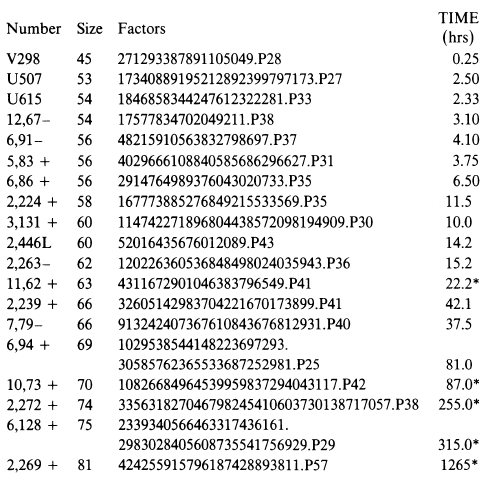
\includegraphics{times}

\section{Параллельная реализация}

Строение алгоритма позволяет легко распараллелить его между машинами, и мы уже сделали это ранее. Центральный процессор выбирает значение $D$ из Части 3 ,и передает его сопроцессору. Сопроцессов вычисляет корни многочленов, выполняет просеивание и возвращает любые найденные факторизации на центральный процессов. Так как все вычисления на сопроцессорах выполняются независимо друг от друга, и так как сопроцессоры коммуницируют только с центральным процессором а не друг с другом, можно достичь максимальной теоретической эффективности всех процессоров. В нашей реализации мы достигли результата с ускорением в $N$ раз при использовании $N$ процессоров. Еще один плюс нескольких сопроцессоров - это сильно увеличенная реальная память. Количество сваппинга и пейджинга уменьшено фактически до нуля, и у нас намного меньше пропусков кэша.

\section{Сравнение с другими методами}

\subsection{Алгоритм на непрерывных дробях}
Алгоритм CFRAC Моррисона и Бриллхарт был чемпионом среди факторизующих алгоритмов вплоть до реализации квадратичного решета Дэвисом. Считалось, что точка пересечения между этими двумя алгоритмами находится где-то между числами из 50 и 70 десятичных знаков.До настоящего момента никто не реализовывал оба эти алгоритма на одной машине. У нас имеется серьезный опыт работы с VAX версией алгоритма CFRAC, которая использует стратегию раннего выхода Померанца, и мы представляем сравнение этих двух методов:


\begin{figure}[H]
\centering
\begin{tikzpicture}
	\pgfplotsset{
		log y ticks with fixed point/.style={
		      yticklabel={
				\pgfkeys{/pgf/fpu=true}
		        	\pgfmathparse{log10(exp((\tick)))}%
		       	\pgfmathprintnumber[fixed relative, precision=3]{\pgfmathresult}
		        	\pgfkeys{/pgf/fpu=false}
			}
		}
	}
	\begin{axis}[
		width=0.8\textwidth,
		height=0.6\textwidth, 
		legend pos=south east,
		ymode=log,
		log y ticks with fixed point,
		yminorticks=false,
		ymax = 1e6,
		xmax = 70,
		xmin = 22,
		xtick = {24, 30, 36, 42, 48, 54, 60, 66},
		xlabel=Размер числа,
		ylabel=$\log{(\text{Время в секундах})}$,
		axis x line*=bottom,
		axis y line*= left]
		\addplot coordinates {
			(24, 10) (30, 240) (36, 2100) (42, 10800) (48, 54000)
		} 
		node[pos=0.27, pin=left:4 мин.]{}
		node[pos=0.52, pin=left:35 мин.]{}
		node[pos=0.75, pin=left:3 ч.]{}
		node[pos=1.0, pin=left:15 ч.]{} ;
		\addplot coordinates {
			(24, 12) (30, 120) (36, 480) (42, 2100) (48, 7200) (54, 28800) (60, 108000) 
		}
		node[pos=0.17, pin=right:2 мин.]{}
		node[pos=0.333, pin=right:8 мин.]{}
		node[pos=0.5, pin=right:35 мин.]{}
		node[pos=0.67, pin=right:2 ч.]{}
		node[pos=0.83, pin=right:8 ч.]{}
		node[pos=1.0, pin=left:30 ч.]{} ;
	\addlegendentry{CFRAC}
	\addlegendentry{MP-QS}
	\end{axis}
	
\end{tikzpicture}
\caption{Сравнение скорости двух алгоритмов}
\label{Рисунок:1}
\end{figure}


Версия квадратичного решета с несколькими многочленами значительно быстрее, как только длина числа становится хоть сколько то большой.Когда берется число $M$ достаточно большое, чтобы наш алгоритм использовал только один многочлен, время работы сильно возрастает. Точка пересечения между этими алгоритмами находится где-то в районе чисел длиной 40 десятичных знаков.

\subsection{Квадратичное решето с одним многочленом}
Мы представляем здесь данные, взятые из \cite{sand}, вместе с нашими собственными данными, которые показывают общее количество вычетов, исследованных вариантами QS. Эти данные представляют типичные значения для общего числа просеянных вычетов как нашим методом, так и методом ''особых $q$'' Дэвиса. Данные значения типичны для чисел данного размера, но столбцы не представляют факторизации одинаковых чисел.

\begin{table}[h!]
	\centering
	\begin{tabular}{ c c c c }
		Размер & MP-QS/VAX &  SPECIAL-Q/CRAY & BASIC-QS/CRAY \\
		52 & 8.0E + 8 & 1.0E + 9K & 9.0E + 9\\
		53 & 4.0E + 8 & - & 2.0E + 10\\
		55 & 5.0E + 8 & - & 1.4E + 10\\
		58 & 1.0E + 9 & 4.3E + 9 & 2.7E + 10\\
		60 & 2.1E + 9 & 2.2E + 10 & 9.0E + 10\\
		63 & 1.0E + 9 & 1.2E + 10 & -
	\end{tabular}
	\caption{Сравнение времени работы разных алгоритмов и компьютеров}
	\label{Таблица:2}
\end{table}

Можно заметить резкое улучшение в сравнении с базовым алгоритмом, и в случае ''особых $q$'' и в нашей версии. Наша версия показала себя несколько лучше по следующим причинам:

\begin{enumerate}[label=\roman*]
	\item Мы использовали множители а Сандия - нет
	\item Мы использовали версию с большими простыми числами
	\item Мы изменяли многочлены так часто как только можно, при использовании большего количества ''особых $q$'' можно было бы улучшить результат Сандии
	\item Архитектура трубопровода, реализованная в Cray относительно быстрее чем VAX, даже принимая во внимание разницу в машинной скорости. Так что более выгодно делать больше просеиваний на каждом многочлене
	\item Наши многчлены производили намного меньшие вычеты

\end{enumerate} 

Эти результаты показывают, что желательно изменять многочлены так часто, как можно. Точное время, затраченное на это, в сравнении с просеиванием будет зависеть от машины и скорее всего требует экспериментов. Изменяя многочлены часто мы получаем как минимум 10 знаков преимущества над базовым алгоритмом, и новые многочлены, представленные нами, дают 1 дополнительный знак.
Автор благодарен Петеру Монтгомери в Корпорации Разработки Систем за предоставление многих советов и предложения, Дж. Дэвису за разрешение на публикацию результатов из таблицы 3, и центру компьютерных исследований в MITRE за предоставление компьютерного времени, использованного в этом проекте.

\nocite{*}

\bibliographystyle{unsrt}
\bibliography{silbib}

\end{document}
